\section{Liquid Level Control System}
\subsection{Liquid level system}
\begin{figure}[htbp]
	\centering
	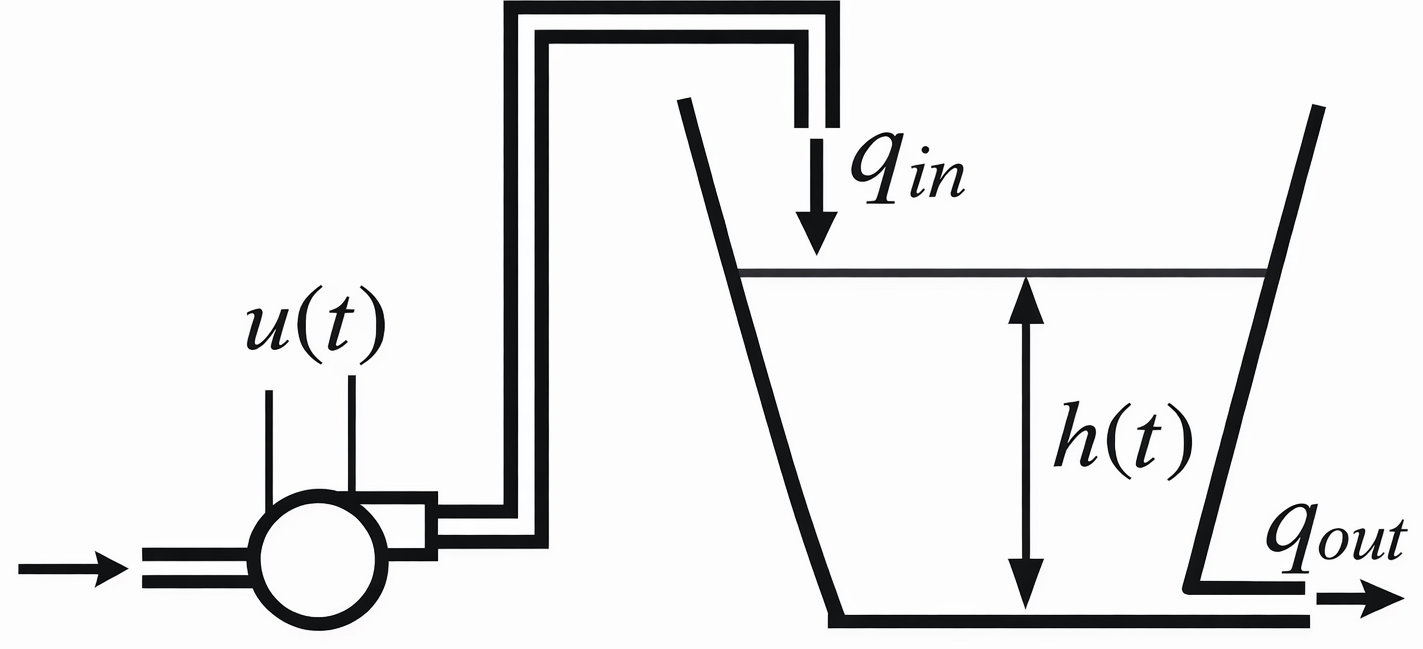
\includegraphics[width=0.45\linewidth]{images/level_control.png}
	\caption{Liquid level control system.}
	\label{fig:level_control}
\end{figure}
\textbf{Requirement:} Design a PID control system with parameters tuned by fuzzy logic, for a water tank plant as shown in \autoref{fig:level_control} so that the water level tracks the desired values as follows:

\begin{equation}
	h(t) = 
	\begin{cases} 
		30 & \text{for } 0\text{ s} < t \le 200\text{ s} \\
		60 & \text{for } 200\text{ s} < t \le 400\text{ s} \\
		90 & \text{for } 400\text{ s} < t 
	\end{cases}
\end{equation}

The dynamic behavior of the water tank is derived from the principle of mass balance. The rate of change of the water volume in the tank is equal to the difference between the inflow rate ($q_{in}$) and the outflow rate ($q_{out}$). Because the tank has a varying cross-sectional area $A(h)$, the rate of change of the water level $\dot{h}$ is defined by the following non-linear differential equation:
\begin{align}
	\dot{h} &= \frac{1}{A(h)} \left( ku(t) - C_D a \sqrt{2gh(t)} \right) \\
	A(h) &= \frac{A_{max} - A_{min}}{h_{max}} h + A_{min}
\end{align}
\noindent System Variables:
\begin{itemize}
	\item $h(t)$: The continuous water level in the tank at time $t$ (System state and output).
	\item $\dot{h}$: The rate of change of the water level over time.
	\item $u(t)$: The control signal applied to the pump (System input).
\end{itemize}

Where the system parameters are:
\begin{itemize}
	\item $h_{max} = 60 \text{ cm}$
	\item $A_{max} = 200 \text{ cm}^2$
	\item $A_{min} = 100 \text{ cm}^2$
	\item $k = 300 \text{ cm}^3/\text{s}$
	\item $a = 1 \text{ cm}^2$
	\item $g = 9.81 \text{ m/s}^2 = 981 \text{ cm/s}^2$
	\item $C_D = 0.6$
\end{itemize}

The PID control law is defined as

\begin{equation}
	u(t) = K_P e(t) + K_I \int_0^t e(\tau)d\tau + K_D \frac{de(t)}{dt}
\end{equation}

where:
\begin{itemize}
	\item $e(t) = r(t) - y(t)$ is the tracking error,
	\item $r(t)$ is the reference (setpoint),
	\item $y(t)$ is the system output,
	\item $K_P$, $K_I$, and $K_D$ are proportional, integral, and derivative gains.
\end{itemize}

In this work, $K_P$ and $K_I$ are tuned online using a Sugeno-type fuzzy inference system (FIS), while $K_D$ is kept constant.

\subsection{Control system design}

Sugeno fuzzy inference system, the controller consists of one input variable, namely the \textit{Setpoint (h(t))}, and two outputs, $K_P$ and $K_I$. The input variable is described by four triangular membership functions corresponding to the linguistic terms: VeryLow, Low, Average, and High. The outputs $K_P$ and $K_I$ are defined as constant consequents, forming a zero-order Sugeno model.

The fuzzy rule base contains four rules, where each operating condition of the setpoint directly determines the proportional and integral gains of the PI controller. The complete fuzzy rule table is presented in \autoref{tab:fuzzy_rule_base}.
\begin{table}[h]
	\centering
	\caption{Fuzzy Logic Rule Base of the Sugeno FIS for tune PI}
	\begin{tabular}{cccc}
		\hline
		\textbf{Rule} & \textbf{Setpoint} & $\mathbf{K_P}$ & $\mathbf{K_I}$ \\
		\hline
		R1 & VeryLow  & 0.90 & 0.08  \\
		R2 & Low      & 0.80 & 0.055 \\
		R3 & Average  & 0.70 & 0.035 \\
		R4 & High     & 0.60 & 0.02  \\
		\hline
	\end{tabular}
	\label{tab:fuzzy_rule_base}
\end{table}
In linguistic form, the rules are expressed as follows:
\begin{itemize}
	\item IF Setpoint is VeryLow THEN $K_P = 0.9$ and $K_I = 0.08$.
	\item IF Setpoint is Low THEN $K_P = 0.8$ and $K_I = 0.055$.
	\item IF Setpoint is Average THEN $K_P = 0.7$ and $K_I = 0.035$.
	\item IF Setpoint is High THEN $K_P = 0.6$ and $K_I = 0.02$.
\end{itemize}


\begin{figure}[t]
	\centering
	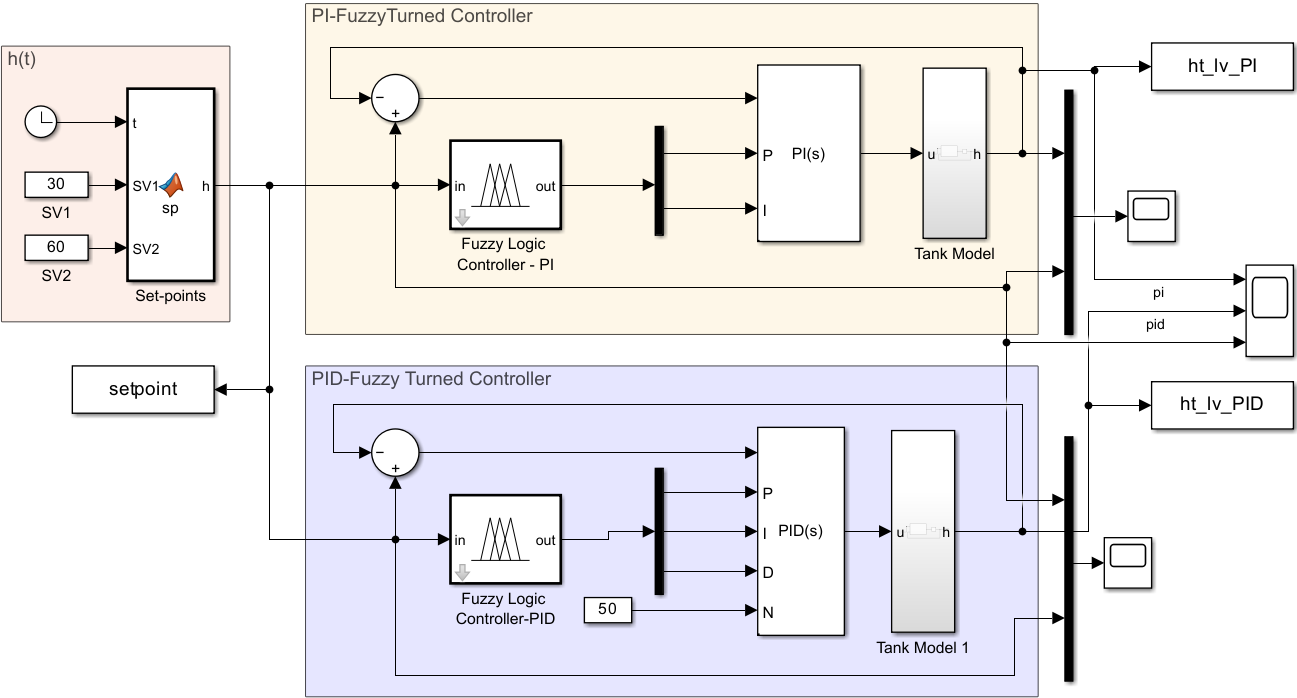
\includegraphics[width=\linewidth]{images/level_control_simulink.png}
	\caption{Simulink block diagram for the design of PI and PID control systems with parameters tuned using fuzzy logic for a water tank plant.}
	\label{fig:level_control_simu}
\end{figure}

\subsection{Simulation Results}
\autoref{fig:all_level_control} illustrates the dynamic response of the water level $h(t)$ under PI and fuzzy-tuned PID control strategies. The reference signal is applied in three step changes at $SV1 = 30$, $SV2 = 60$, and $SV1+SV2 = 90$. Both controllers successfully track the setpoint with fast rise time and minimal steady-state error. However, the fuzzy-tuned PID controller exhibits slightly improved transient performance, including reduced overshoot and faster settling time compared to the PI controller. These results demonstrate the effectiveness of fuzzy logic tuning in enhancing the overall control performance of the water tank system.
\begin{figure}[ht]
	\centering
	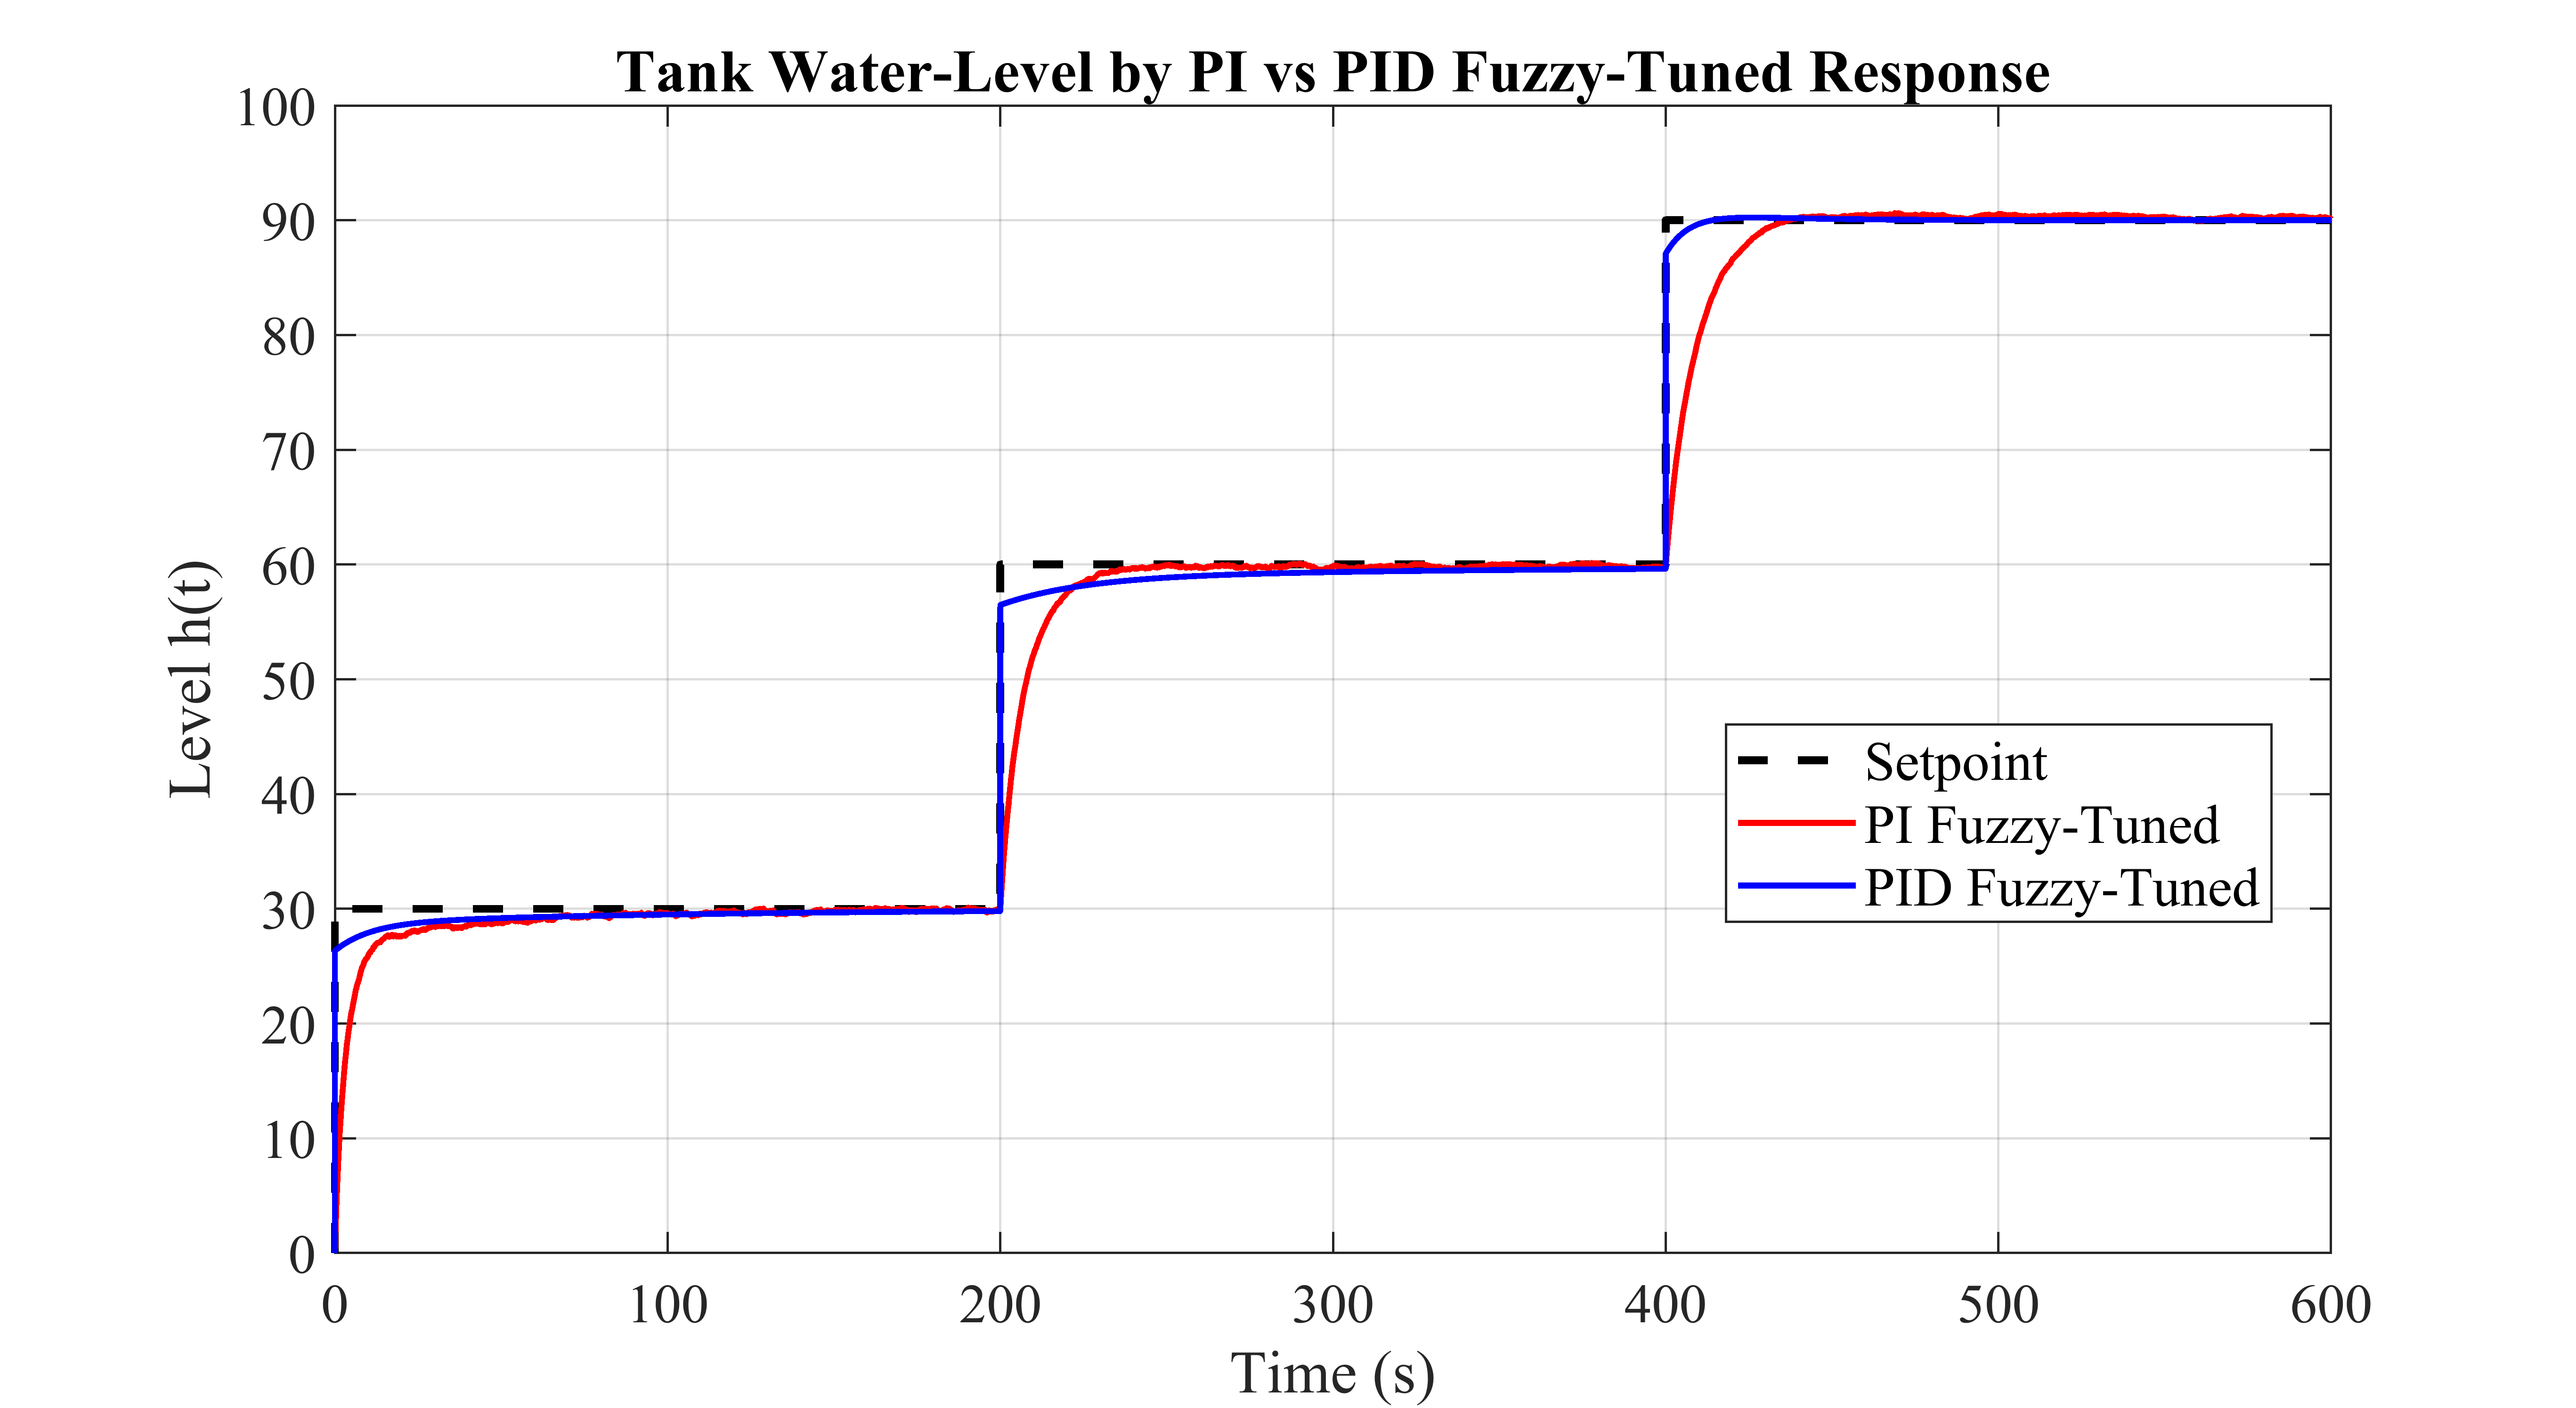
\includegraphics[width=\linewidth]{images/all_level_control_.png}
	\caption{The simulation result of the water level control using PI and fuzzy-tuned PID controllers, as desired, is represented by the function $h(t)$.}
	\label{fig:all_level_control}
\end{figure}

\autoref{fig:30_level_control} presents a detailed view of the transient response of the water level $h(t)$ when the reference signal increases to $SV1 = 30$. Both the fuzzy-tuned PI and fuzzy-tuned PID controllers track the setpoint effectively with negligible steady-state error. The fuzzy-tuned PID controller achieves a faster rise time and slightly smaller overshoot compared to the PI controller, resulting in improved settling performance. This close-up response confirms the enhanced dynamic behavior provided by fuzzy logic tuning in the PID scheme.
\begin{figure}[ht]
	\centering
	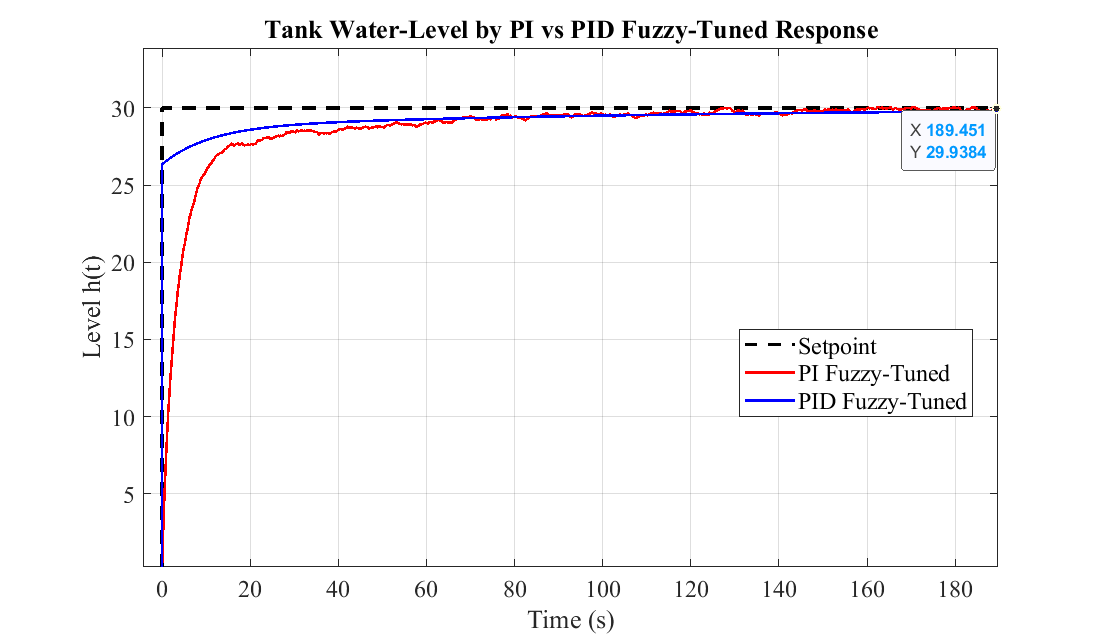
\includegraphics[width=\linewidth]{images/30_level_control.png}
	\caption{The simulation results of water level control using fuzzy-corrected PI and PID controllers show that when $h(t)$ increases to the setpoint value $SV{1} = 30$.}
	\label{fig:30_level_control}
\end{figure}
\autoref{fig:60_level_control} illustrates the transient response of the water level $h(t)$ when the reference signal increases to $SV_1 = 60$. Both fuzzy-tuned PI and fuzzy-tuned PID controllers successfully track the new setpoint with negligible steady-state error. 
\begin{figure}[ht]
	\centering
	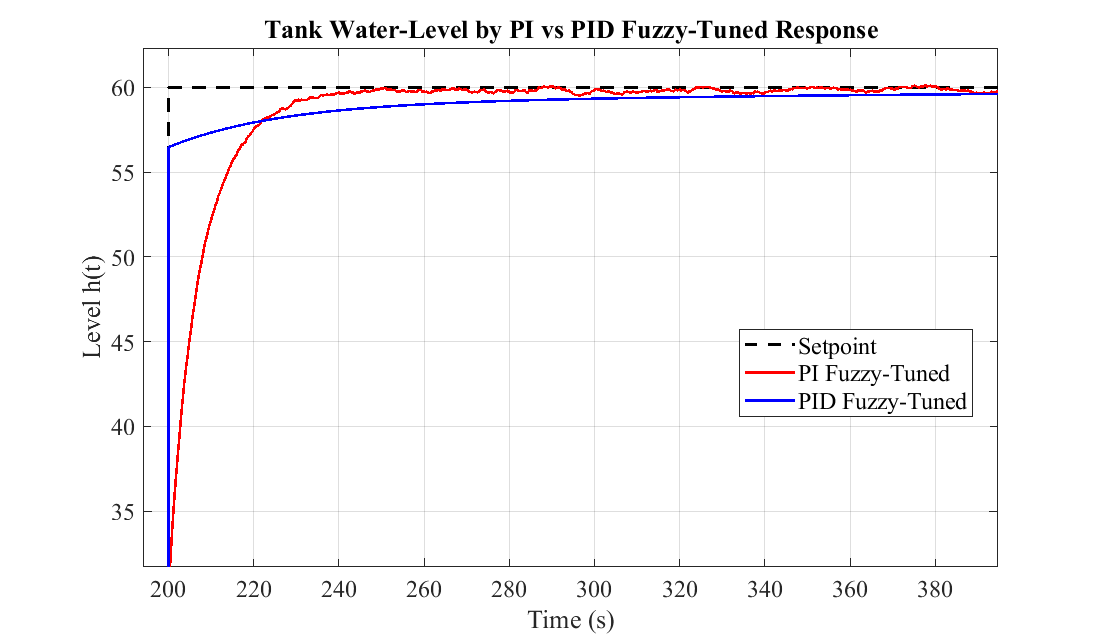
\includegraphics[width=\linewidth]{images/60_level_control.png}
	\caption{The simulation results of water level control using fuzzy-corrected PI and PID controllers show that when $h(t)$ increases to the setpoint value $SV{1} = 60$.}
	\label{fig:60_level_control}
\end{figure}
\begin{figure}[ht]
	\centering
	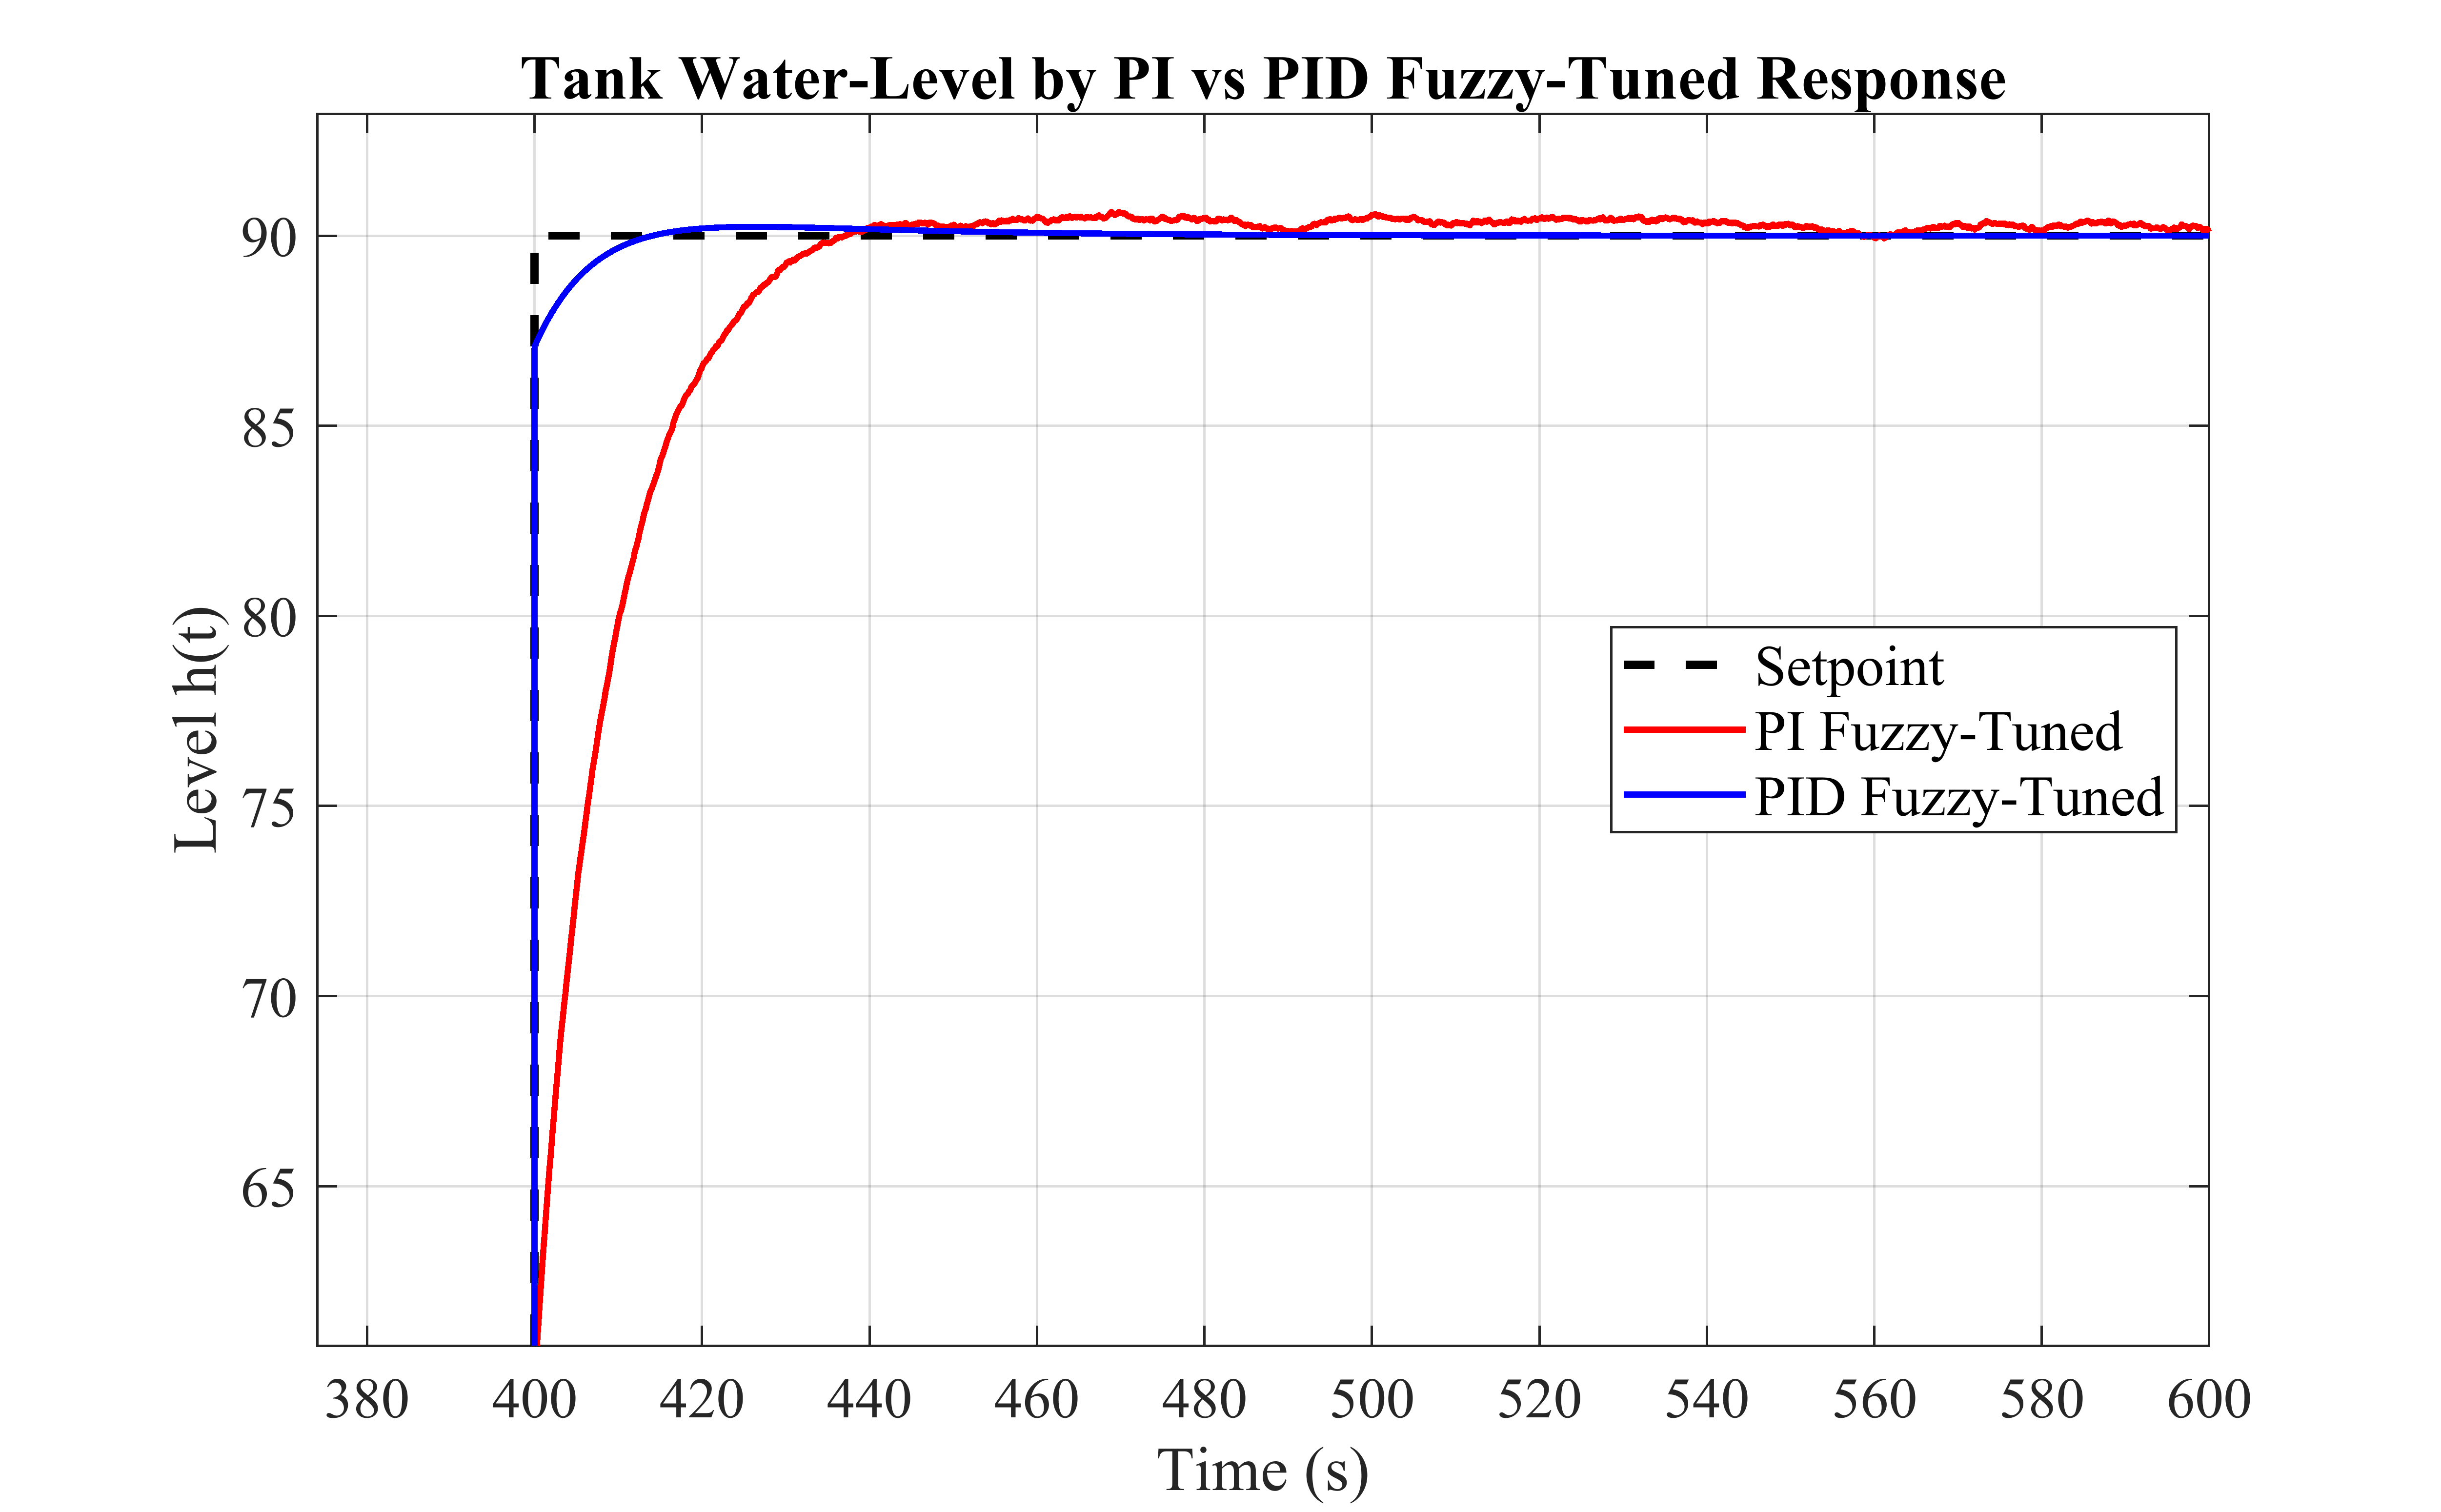
\includegraphics[width=\linewidth]{images/90_level_control.png}
	\caption{The simulation results of water level control using fuzzy-corrected PI and PID controllers show that when $h(t)$ increases to the setpoint value $SV{1} + SV{2} = 90$.}
	\label{fig:90_level_control}
\end{figure}
\autoref{fig:90_level_control} presents the transient response of the water level $h(t)$ when the reference signal increases to $SV_1 + SV_2 = 90$. Both fuzzy-tuned PI and fuzzy-tuned PID controllers accurately track the setpoint with negligible steady-state error. 
These results indicate that the fuzzy-tuned PID controller significantly reduces overshoot and provides smoother transient behavior compared to the PI controller, confirming the superior dynamic performance achieved through fuzzy logic tuning.

